\section{Addressing Modes}\label{subsec:addressing-modes}
\par Any addressing mode can be applied to instructions that need a data source.
The addressing mode determines how that data will be obtained.

\subsection{Immediate}\label{subsec:immediate-(imm)}
\subsubsection{Syntax}
\begin{verbatim}[operation].imm [8-bit immediate]\end{verbatim}

\subsubsection{Description}
$OperandValue = SignExtend(Immediate)$
\par The 8-bit operand field will be sign-extended to 16-bits.
It will then immediately be used as the secondary operand for the instruction.

\subsubsection{Encoding}
\begin{center}
    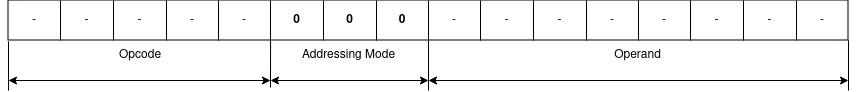
\includegraphics[scale=0.40]{img/Andromeda-IMM.drawio}
\end{center}

\subsubsection{Example}
\begin{verbatim}

        org(0x0000)
    def entry:
        lda.imm     -12
        hlt

\end{verbatim}
The code above would result in `-12' being loaded into the accumulator.
The 16-bit two's complement form of -12 is $1111111111110100_{2}$.
This value is the sign-extended version of the 8-bit value `$1111010_{2}$' that was embedded in the instruction's operand field.
\pagebreak

\subsection{Memory Direct}\label{subsec:memory-direct-(dir)}
\subsubsection{Syntax}
\begin{verbatim}[operation].dir [8-bit immediate]\end{verbatim}

\subsubsection{Description}
$OperandValue = Memory[FF00_{16} + Immediate]$
\par The constant $FF00_{16}$ will be added to the 8-bit operand field.
This will yield a 16-bit value in the range $FF00_{16}$ - $FFFF_{16}$ inclusive.
This value will then be used as an address.
The value stored at that address will be used as the secondary operand for the instruction.

\subsubsection{Encoding}
\begin{center}
    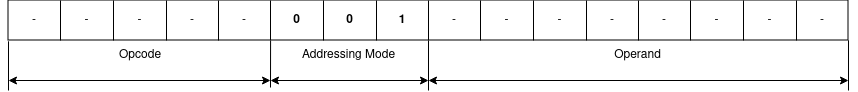
\includegraphics[scale=0.40]{img/Andromeda-DIR.drawio}
\end{center}

\subsubsection{Example}
\begin{verbatim}

        org(0x0000)
    def entry:
        sta.dir     0x01
        hlt

\end{verbatim}
The code above would store the accumulator into the address $FF01_{16}$.
\pagebreak

\subsection{Relative Memory Direct}\label{subsec:relative-direct-(rel)}

\subsubsection{Syntax}
\begin{verbatim}[operation].rel [8-bit immediate]\end{verbatim}

\subsubsection{Description}
$OperandValue = Memory[PC + SignExtend(Immediate)]$
\par The 8-bit operand field is sign-extended to 16-bits.
That value is added to the program counter (PC) to yield and address.
The contents of that address will be used as the secondary operand for the instruction.

\subsubsection{Encoding}
\begin{center}
    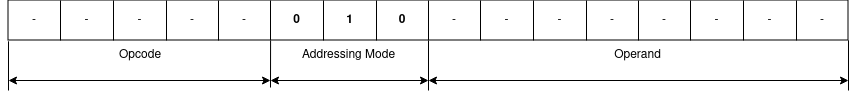
\includegraphics[scale=0.40]{img/Andromeda-REL.drawio}
\end{center}

\subsubsection{Example}
\begin{verbatim}

        org(0x0000)
    def entry:
        nop
        lda.rel     2
        hlt
    def data:
        dw(-11)

\end{verbatim}
The code above would be result in -11 being loaded into the Accumulator.
The `lda' instruction exists at address $0001_{16}$, adding `2' to this address results in the value $0003_{16}$.
The value stored at $0003_{16}$ (`-11') is loaded into the Accumulator.
\pagebreak

\subsection{Offset}\label{subsec:relative-jump}
\subsubsection{Syntax}
\begin{verbatim}[operation].off [8-bit immediate]\end{verbatim}

\subsubsection{Description}
$OperandValue = PC + SignExtend(Immediate)$
\par The 8-bit operand field is sign-extended to 16-bits.
That value is added to the program counter (PC) to yield the operand value.

\subsubsection{Encoding}
\begin{center}
    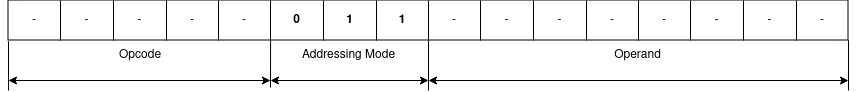
\includegraphics[scale=0.40]{img/Andromeda-OFF.drawio}
\end{center}

\subsubsection{Example}
\begin{verbatim}

    org(0x0000)
def entry:
    lda.imm     100
    jmp.off     2
    lda.imm     200
    hlt

\end{verbatim}
The code above would result in `$100_{10}$' in the Accumulator.
The \texttt{jmp.off 2} exists at address $0001_{16}$.
Adding $0002_{16}$ to that address results in address $0004_{16}$, where the halt instruction exists.
As a result, Tth \texttt{jmp.off 2} instruction skipped the `\texttt{lda.imm 200}' instruction.
This means only the first `\texttt{lda.imm 100}' instruction was executed.
\pagebreak

\subsection{Memory Indirect}\label{subsec:memory-indirect-(ind)}
\subsubsection{Syntax}
\begin{verbatim}[jump operation].ind [8-bit immediate]\end{verbatim}

\subsubsection{Description}
$OperandValue = Memory[Memory[FF00_{16} + Immediate]]$
\par The constant $FF00_{16}$ will be added to the 8-bit operand field.
This will yield a 16-bit value in the range $FF00_{16}$ - $FFFF_{16}$ inclusive.
This value will then be used as an address.
The value stored at that address will be used as another address known as the pointer.
This value stored at this final pointer address will be used as the secondary operand for the instruction.

\subsubsection{Encoding}
\begin{center}
    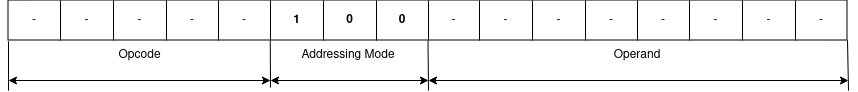
\includegraphics[scale=0.40]{img/Andromeda-IND.drawio}
\end{center}

\subsubsection{Example}
\begin{verbatim}

        org(0x0000)
    def entry:
        lda.ind pointer
        hlt

        org(0xFF01)
    def pointer:
        0xD000

        org(0xD000)
    def final_value:
        -12

\end{verbatim}
The code above will result in -12 being loaded into the accumulator.
The value stored in address $FF01_{16}$ ($D000_{16}$) was used as an address to find the final value (-12).
\pagebreak

\subsection{Memory Indirect \& Auto Increment}\label{subsec:memory-indirect-&-auto-increment-(inc)}
\subsubsection{Syntax}
\begin{verbatim}[jump operation].inc [8-bit immediate]\end{verbatim}

\subsubsection{Description}
$OperandValue = Memory[Memory[(FF00_{16} + Immediate)++]]$\\
\par This addressing mode behaves similarly to memory indirect addressing.
The secondary operand is obtained in the same manner.
However, after the value is obtained, the pointer will be incremented.

\subsubsection{Encoding}
\begin{center}
    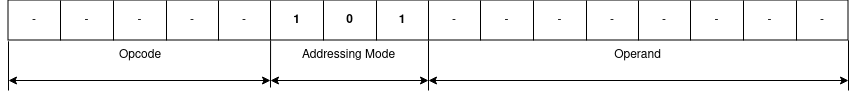
\includegraphics[scale=0.40]{img/Andromeda-INC.drawio}
\end{center}

\subsubsection{Example}
\begin{verbatim}

        org(0x0000)
    def entry:
        lda.inc pointer
        hlt

        org(0xFF01)
    def pointer:
        0xD000

        org(0xD000)
    def final_value:
        -12

\end{verbatim}
The code above will result in -12 being loaded into the accumulator.
However, after the instruction has completed execution, pointer will be incremented to $D001_{16}$
\pagebreak

\subsection{Auto Decrement \& Memory Indirect}\label{subsec:auto-decrement-&-memory-indirect-(dec)}
\subsubsection{Syntax}
\begin{verbatim}[jump operation].dec [8-bit immediate]\end{verbatim}

\subsubsection{Description}
$OperandValue = Memory[Memory[--(FF00_{16} + Immediate)]]$
\par This addressing mode behaves similarly to memory indirect addressing.
Before the instruction is executed, the pointer will be decremented.
Then the secondary operand is obtained in the same manner as it is in simple Memory Indirect addressing.

\subsubsection{Encoding}
\begin{center}
    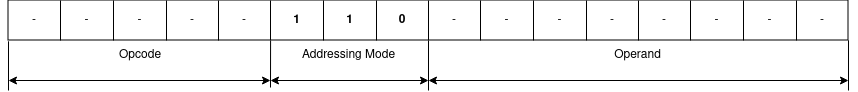
\includegraphics[scale=0.40]{img/Andromeda-DEC.drawio}
\end{center}

\subsubsection{Example}
\begin{verbatim}

        org(0x0000)
    def entry:
        lda.dec pointer
        hlt

        org(0xFF01)
    def pointer:
        0xD001

        org(0xD000)
    def final_value:
        13
        -12

\end{verbatim}
The code above will result in 13 being loaded into the accumulator.
Pointer will have been decremented to $D000_{16}$ so the `13' could be addressed indirectly
\pagebreak

\subsection{Reference Card}\label{subsec:reference-card}
\renewcommand{\arraystretch}{2.0}
\begin{center}
    \begin{adjustbox}{width=\textwidth}
        \begin{tabular}{ |c|c|c| }
            \hline
            Mnemonic & Operand Value & Encoding \\ \hline
            \texttt{imm} & $SignExtend(Immediate)$ & $000_{2}$ \\ \hline
            \texttt{dir} & $Memory[FF00_{16} + Immediate]$ & $001_{2}$\\ \hline
            \texttt{rel} & $Memory[PC + SignExtend(Immediate)]$ & $010_{2}$\\ \hline
            \texttt{off} & $PC + SignExtend(Immediate)$ & $011_{2}$\\ \hline
            \texttt{ind} & $Memory[Memory[FF00_{16} + Immediate]]$ & $100_{2}$\\ \hline
            \texttt{inc} & $Memory[Memory[(FF00_{16} + Immediate)++]]$ & $101_{2}$\\ \hline
            \texttt{dec} & $Memory[--(Memory[FF00_{16} + Immediate)]]$ & $110_{2}$\\ \hline
        \end{tabular}
    \end{adjustbox}
\end{center}

Note: The table above uses the C/C++ convention for postfixing and prefixing increments (\texttt{++}) and decrements (\texttt{--}).
\par If the operator appears before the value, the operation is performed before the value is calculated.
If the operator appears after the value, the operation is performed after the value is calculated.
